\chapter{Viscosità}
\section{Introduzione}
\subsection{Obiettivo di ricerca}
L'obiettivo della ricerca è misurare l'indice di viscosità della glicerina. Questo risultato sarà raggiunto tramite la misura dei tempi di caduta di una serie di sferette di acciaio di diverse dimensioni all'interno di un cilindro riempito di glicerina. 

\subsection{Strumenti di laboratorio}
Il diametro della sfere è stato misurato con un calibro, e l'incertezza associata alla misura è di $\pm0.05 mm$. Il peso è stato misurato con una bilancia, e l'incertezza associata alla misura è  $\pm10^{-6}$ kg.
La densità del liquido è il valore tabulato :  $\rho_{liquido} =  1260.0\  kg/m^3 $, scelto a 25 C°
\begin{center}
\begin{tabular}{ll |c}
& Massa ($g$)& $\rho_{sfera} \ (kg/m^3)$\\
\midrule
 \textbf{Sferette da 3mm:}
 & 0.110 & 7780.91 \\
 \midrule
\textbf{Sferette da 4mm: }
 & 0.261 & 7788.65\\
 \midrule
\textbf{Sferette da 5mm: }
 & 0.510 & 7792.23 \\
 \midrule
 \textbf{Sferette da 6mm:}
  & 0.880 & 7780.91\\
  \midrule
  & $\-{\rho_{sfera}}$& 7785.65\\
\end{tabular}
\end{center}
Conservando le tre cifre significative iniziali ottengo un $\-{\rho_{sfera}} = \ 7.79 \cdot 10^3 \ kg/m^3$
\\

Ai fini dell'esperimento, le incertezze associate alle misure della massa e del diametro sono state considerate trascurabili, essendo sufficientemente piccole. Nell'analisi dei dati verranno quindi considerate solo le incertezze dovute all'analisi statistica dei tempi misurati. 
\\

Il set-up per l'esperimento è costituto da un cilindro graduato riempito di glicerina, e  da un cronometro digitale. L'incertezza associata a quest'ultimo strumento è $\pm0.01s$. Abbiamo quindi segnato due tacche sul cilindro graduato, per facilitare la lettura del tempo di caduta, poste ad una distanza di $15.1 cm$, distanza misurata con un metro a nastro di sensibilità $\pm 1mm$.

\subsection{Contenuti teorici}
La viscosità è l'attrito dinamico che si oppone al moto di un corpo all'interno di un fluido. Per un moto laminare, la forza di attrito è proporzionale alla velocità e alle caratteristiche del corpo secondo la seguente formula:

$$F_{res} = 6 \pi r v \eta $$

con \textbf{r}  raggio del corpo,\textbf{ v} velocità e $\nu$ indice di viscosità del fluido. 
Per calcolare questo coefficiente di viscosità, si può misurare quindi la velocità del corpo nel fluido, che ad un certo punto risulterà costante. La sommatoria delle forze agenti sul corpo è quindi uguale a zero

$$ R = F_{peso} - F_{archimede} - F_{res} = 0 $$
Da questa uguaglianza si ricava:
\\
\begin{equation}\label{eta}
\eta= 2 g r^2\frac{(\rho_{sfera} - \rho_{liquido})}{9v_{limite}}
\end{equation}

Per ricavare la velocità limite, si divide la distanza percorsa per il tempo di caduta. 

\section{Raccolta dati}
Di seguito le tabelle che registrano il tempo di caduta delle sfere.
\subsubsection{Sferette da 6mm}
\begin{tabular}{c|c|c|c|c|c|c|c|c|c}
\toprule
 1,68s & 1,68s & 1,65s & 2,21s* & 1,68s & 1,68s & 1,62s & 1,71s & 1,71s & 1,75s \\
 1,78s & 1,71s & 1,71s & 1,65s & 1,59s  & 1,65s  & 1,71s  & 1,68s & 1,68s & 1,65s \\
\midrule
 1,62s & 1,56s & 1,71s & 1,71s & 1,68s & 1,62s & 1,59s & 1,59s & 1,53s & 1,59s \\
 1,46s & 1,62s & 1,59s & 1,56s & 1,62s & 1,56s & 1,62s & 1,43s & 1,53s & 1,59s \\
\midrule
 1,56s & 1,56s & 1,53s & 1,62s & 1,68s & 1,56s & 1,56s & 1,59s & 1,59s & 1,50s\\
 1,53s & 1,62s & 1,50s & 1,56s & 1,59s & 1,62s & 1,43s & 1,62s & 1,43s & 1,40s \\
\midrule
 1,59s & 1,46s & 1,46s & 1,59s & 1,65s & 1,59s & 1,68s & 1,43s & 1,53s & 1,62s \\
 1,46s & 1,50s & 1,56s & 1,59s & 1,50s & 1,59s  & 1,59s & 1,59s & 1,53s & 1,59s \\
\midrule
1,59s & 1,46s & 1,53s & 1,43s & 1,53s & 1,46s & 1,46 & 1,56 & 1,40s & 1,34s \\
1,46s & 1,37s  & 1,50s   & 1,50s  & 1,43s & 1,31s & 1,40s  & 1,43s  & 1,34s & 1,43s \\
\bottomrule
\end{tabular}
\subsubsection{Sferette da 5mm}
\begin{tabular}{c|c|c|c|c|c|c|c|c|c}
\toprule
 2,34s* & 2,43s* & 2,31s & 2,21s & 2,12s & 2,53s* & 2,21s & 2,21s & 2,71s* & 2,71s* \\
 2,12s & 2,34s & 2,18s & 2,34* & 2,12s & 2,06s & 2,12s & 2,59s* & 2,03s & 2,06s \\
\midrule
 2,87s* & 2,21s & 2,21s & 2,12s & 2,03s & 2,09s & 2,12s & 2,46* & 2,06s & 2,25s \\
 2,15s & 2,25s & 2,00s &  &  &  &  &  &  & \\
\bottomrule
\end{tabular}
\subsubsection{Sferette da 4mm}
\begin{tabular}{c|c|c|c|c|c|c|c|c|c}
\toprule
 3,06s & 3,09s & 3,15s & 3,12s & 3,03s & 3,15s & 3,25s & 3,25s & 3,18s & 3,09s \\
 3,09s & 3,09s & 3,21s & 3,12s & 3,06s & 3,06s & 3,15s & 3,46s & 3,25s & 3,12s \\
\bottomrule
\end{tabular}
\subsubsection{Sferette da 3mm}

\begin{tabular}{c|c|c|c|c|c|c|c|c|c}
\toprule
 5,28s & 5,09s & 4,96s & 5,25s & 5,28s & 5,12s & 5,06s & 5,12s & 5,06s & 5,28s \\
 5,03s & 5,06s & 4,87s & 4,90s & 4,96s & 5,06s & 5,06s & 4,95s & 4,93s & 5,18s \\
 5,18s & 5,18s & 5,21s & 4,87 & 5,34s &  &  &  &  & \\
\bottomrule
\end{tabular}


* = per queste misurazioni, la pallina si è avvicinata molto alla parete del tubo, e dunque le misurazioni potrebbero essere falsate.
Per le sferette da 6mm abbiamo scartato il valore 2.21s, connotato dall'asterisco, perchè esso dista circa 6.5 deviazioni standard dal valore medio.

\section{Calcolo dei tempi}
Di seguito, gli istogrammi relative alle misure con la gaussiana associata:
\\
\includegraphics[scale=0.4]{"../grafici/5mm"}
\includegraphics[scale=0.4]{"../grafici/6mm"}
Mostriamo solo gli istogrammi e la gaussiana delle sfere da 5 e da 6 mm perchè hanno un numero di misure significativo per mostrare una distribuzione corretta.

\section{Calcolo delle velocità}
Per calcolare la velocità, si divide la distanza ( $ d= 15.1\ cm$) per il tempo medio calcolato in precedenza:
$$ v_{limite} = \frac{d}{t_{\mu}} $$
L'incertezza sulle due misure si propaga secondo la seguente formula, con $\sigma_d=20\ cm$
\begin{equation}
 \frac{\sigma v}{v} = \sqrt{\left(\frac{\sigma d}{d}\right)^2 + \left(\frac{\sigma_t}{t}\right)^2} 
\end{equation}

\begin{center}
\begin{tabular}{c|c|c|c|c}
Sfera & Tempo ($s$) & $\sigma_t\ (s) $ & Velocità ($m/s$) & $\sigma_v \ (m/s) $\\
\midrule
3mm & 5.09 & 0.13 & 2.96 & 0.08\\
4mm & 3.15 & 0.10 & 4.79 & 0.15\\
5mm & 2.16 & 0.11 & 6.99 & 0.36\\
6mm & 1.56 & 0.10 & 9.68 & 0.62\\
\end{tabular}
\end{center}
La relazione tra la velocità e il raggio può essere vista con maggior chiarezza se riscriviamo \ref{eta}  in questo modo: 
\begin{equation}\label{vlim}
v_{limite}=  \frac{2g(\rho_{sfera} - \rho_{liquido})}{9 \eta} \cdot r^2
\end{equation}
La velocità dipende quindi linearmente dal raggio quadratico.
\begin{center}
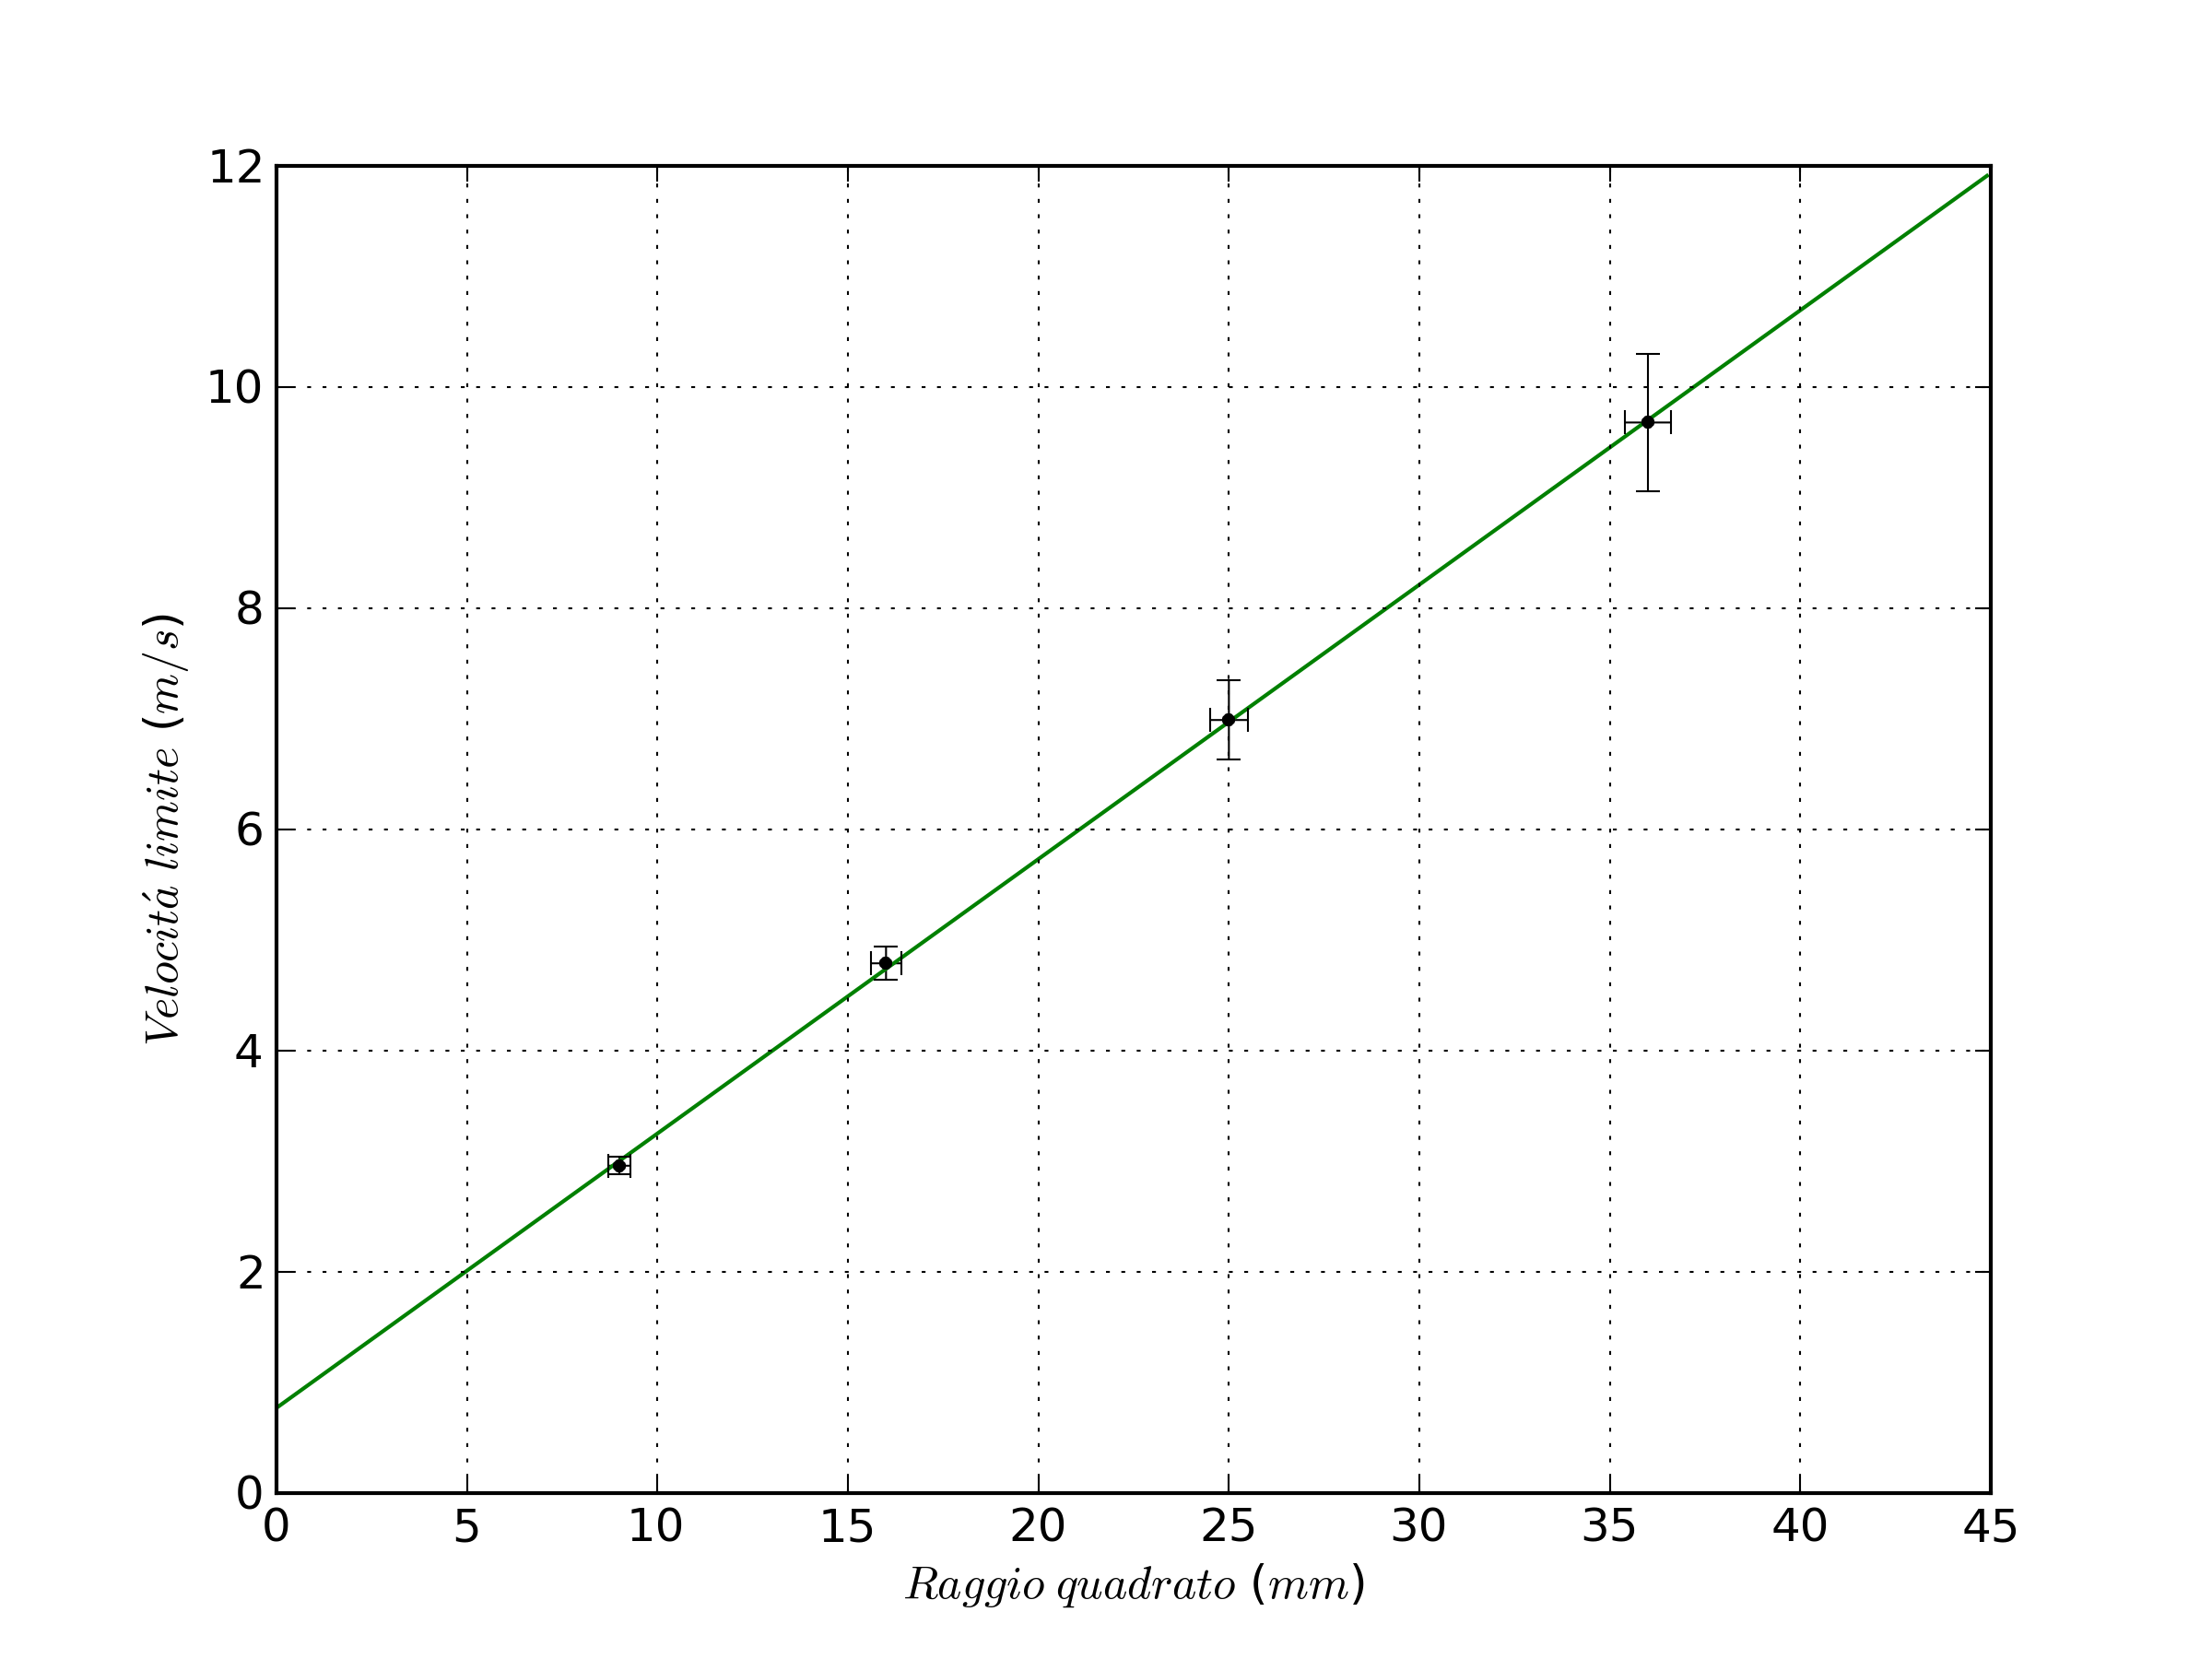
\includegraphics[scale=0.75]{../grafici/velocita}
\end{center}
Notiamo che il coefficiente angolare $m$ dell'equazione \label{vlim} è dato da:
\begin{equation}
m= \frac{2g(\rho_{sfera} - \rho_{liquido})}{9 \eta}
\end{equation}
Conoscendo il valore numerico di $m$ , possiamo ricavare il coefficiente di viscosità.

\begin{equation}
\eta = \frac{2g(\rho_{sfera} - \rho_{liquido})}{9 m}
\end{equation}
Con $m = 9.92 \cdot 10^{5} m^{-1}\cdot s^{-1}$ otteniamo  $\eta = 1.4344 \ Pa \cdot s$.
Il valore tabulato per la glicerina a 20C  è di $1.412 Pa \cdot s$. Abbiamo quindi raggiunto un risultato in accordo con la teoria. 

\subsection*{Errore sistematico}
La retta che interpola i dati non passa dall'orgine. L'equazione \ref{vlim} è infatti una relazione lineare con $q=0$. Il discostamento della retta prevista rispetto a  quella che effettivamente interpola i dati potrebbe essere dovuto ad un errore sistematico che si è ripetuto su tutte le misure. L'entità di questo errore  è $q =0.77 \ m/s$. Nel corso dell'esperimento abbiamo quindi sovvrastimato la velocità di circa $0.77 \ m/s$. Questo errore però non inficia i risultati precedentemente ottenuti: il coefficiente angolare delle due rette è il medesimo, e quindi lo è anche il coefficiente di viscosità.

\section{Conclusioni}
Abbiamo 
